\documentclass[a4paper,twocolumn]{article}

\usepackage[francais]{babel}
\usepackage[T1]{fontenc}
\usepackage{amsmath}
%\usepackage{float}
%\usepackage[top=4cm,bottom=4cm,right=2.5cm,left=2.5cm]{geometry}
\usepackage{color}
\usepackage{tikz}
\usepackage{subfig}
\usepackage{graphicx}
\usepackage[french,ruled,noend]{algorithm2e}
\usepackage[adobe-utopia]{mathdesign}
\usepackage{url}
\usepackage{biblatex}

% Couleurs inspirées de famfamfam.com
\definecolor{vert}{HTML}{59FF2D}
\definecolor{bleu}{HTML}{0BCEFF}
\definecolor{rose}{HTML}{FF0B5B}
\definecolor{gris}{gray}{0.5}

\usetikzlibrary{shapes,fit,calc,3d}

\tikzset{line/.style={
    shorten >= -#1,
    shorten <= -#1}}
\tikzset{halfline/.style={
    shorten >= -#1}}
\tikzset{axe/.style={
    ->,
    thin}}
\tikzset{fig/.style={
    thick}}
\tikzset{origine/.style={
    draw=black,
    cross out}}
\tikzset{aabb/.style={
  dashed,
  thick,
  inner sep=0}}
\tikzset{gjknode/.style={
    fill=rose,
    circle}}
\tikzset{gjkedge/.style={
    draw=rose,
    thick}}
\tikzset{gjkdir/.style={
    halfline=0.5cm,
    draw=gris,
    very thick,
    dashed}}
\tikzset{gjkclosest/.style={
    circle,
    fill=bleu}}
\tikzset{rayon/.style={
    ->,
    dashed,
    draw=gris}}

\newcommand{\deriv}{\partial \!}

\title{Simulation physique de corps rigides avec interaction}
\author{Merwan Achibet}
\date{}

\bibliography{references.bib}

\begin{document}

\shorthandoff{!} % Pour éviter bug de Tikz + Babel french

\maketitle

\tableofcontents
\section{Introduction}

\subsection{Les moteurs physiques}

Invisibles, les phénomènes physiques qui régissent le fonctionnement de notre univers sont pourtant omniprésents et universels. \'Etudiées depuis des siècles, les lois les décrivant ont été à maintes reprises redéfinies et affinnées et il est de nos jours indispensable de pouvoir les modéliser de façon fidèle ou tout du moins d'être capable de les approximer de façon plausible. 

Une simulation industrielle visant par exemple à reproduire virtuellement les interactions entre les différentes pièces qui composent une automobile doit être capable de reproduire de façon réaliste la friction des pneumatiques sur le sol, l'influence de la gravité sur le véhicule, le comportement thermique et volumique des fluides qu'il contient ainsi que de nombreux autres aspects de son fonctionnement. Le système informatique simulant tous ces facteurs est appellé moteur physique. Dans cet exemple, les enjeux de sécurité et de qualité sont grands et des résultats d'une précision extrême sont exigés. Les calculs à mettre en jeu pour les obtenir peuvent donc se permettre d'être très coûteux et de se baser sur des modélisations mathématiques complexes. Il n'est pas rare que ces processus de simulation soient répartis sur plusieurs machines et s'étalent sur une durée de calcul de plusieurs heures.

A contrario, les moteurs physiques d'autres types de système complexe ne peuvent se permettre une telle latence et doivent fonctionner en temps réel. La contrainte est encore plus forte lorsque le moteur physique doit cohabiter avec d'autres modules gérant différents aspects de l'application. On pense notamment aux jeux vidéo, qui partagent le temps de calcul alloué entre le moteur graphique, le moteur d'intelligence artificielle, la gestion du son, la gestion du réseau, et bien sûr le moteur physique. Dans le cadre de ce type d'application, auquel on peut greffer la réalité virtuelle et ses applications dérivées, la contrainte la plus importante est le temps d'éxecution et non la précision des résultats. On ne cherche plus à obtenir des données exactes mais une représentation plausible du réel. Ainsi, certains raccourcis pourront être tolérés et une part de réalisme est sacrifiée au profit de la vitesse.

La physique est un champ très vaste dont les disciplines vont de l'acoustique à l'électronique. Néanmoins, le spectre d'action des moteurs physiques se limite à la mécanique classique, dite mécanique newtonienne. Ce sous-domaine répond à des questions telles que : Comment réagira cette balle si on la lance sur un mur ? Quelle est l'influence d'une planète sur un objet spatial donné ? Pourquoi un liquide visqueux dispose-t-il d'une faible vitesse d'écoulement ? Quelles déformations engendrera un choc entre deux voitures ?

La mécanique newtonienne est elle-même une vaste discipline et la précision d'une modélisation ne suffit pas à la différenciation entre tous les moteurs physiques. Souvent, un moteur physique sera spécialisé. Certains simuleront les interactions entre corps rigides comme une boîte en plastique tombant sur le sol. Certains simuleront le comportement d'objets déformables comme une balle de caoutchouc jetée sur un mur. D'autres se concentreront sur les réactions entre liquides ou entre gaz.

\subsection{Travail à accomplir}

L'objectif de ce projet est de concevoir un moteur physique de base permettant de gérer les interactions entre corps rigides convexes. On parle de corps rigides dans la mesure o\`u les objets mis en jeu seront indéformables et incassables. Dans un tel contexte, une tasse en porcelaine surmontée d'un bloc de granite d'une tonne ne serait aucunement endommagée. On parle de corps convexes car se limiter dans un premier temps à ce type de structure autorise certaines facilités dans les calculs. Une piste pour étendre la simulation aux solides concaves sera présentée dans la dernière partie.

La contrainte principale de notre application sera le temps. On veut concevoir une simulation éxecutable en temps réel de telle façon que si l'utilisateur modifie l'environnement de la simulation à un instant quelconque, une réaction à cette interaction soit immédiatement générée. Certains raccourcis dans les calculs ainsi que plusieurs approximations seront acceptés. Le fonctionnement du moteur se base néanmoins sur des lois bien connues de la mécanique de Newton et ses résultats ne devront pas s'éloigner de façon demesurée de ceux que l'on retrouverait dans une situation réelle.

\subsection{\'Etude de cas}

L'activité physique d'un corps se divise en plusieurs phases. Afin de les détailler, analysons une situation concrète. Si l'on tenait une balle dans notre main et que nous la lachions au dessus d'un plan faiblement incliné, quelles seraient les étapes que cet objet traverserait avant d'arriver à un état de repos ?

\subsubsection{La chute}

La main s'ouvre et laisse s'échapper la balle. Notre appréhension du monde qui nous entoure nous permet de prévoir que l'objet tombera et accélérera vers le bas. Ce phénomène est quantifié par la seconde loi de Newton.

\begin{align*}
  \vec{a} = \frac{1}{m} \sum{\vec{F}_i}
\end{align*}

Cette règle décrit l'accélération $\vec{a}$ d'un corps comme étant le produit de l'inverse de sa masse $m$ et de la somme des forces $\vec{F}_i$ qui lui sont appliquées. Dans notre exemple, on lache la balle sans lui donner d'élan initial et la seule influence qu'elle subit au cours de sa chute est celle de la gravité. La gravité terrestre est une force de $9.81 N$ dirigée vers le noyau de la planète mais dans la simulation, on peut la réduire à une force dirigée vers le "bas" (dans la direction négative de l'axe $y$). Afin de bénéficier d'un moteur physique versatile, la puissance de la gravité pourra être modifiée, pour simuler une situation lunaire par exemple, ou être totalement annulée, pour simuler une situation en apesanteur. En réalité, la gravité ne sera pas codée "en dur" mais appartiendra à une liste de forces environnementales qui contiendra toutes les influences que le monde extérieur applique aux objets qu'il contient. On pourra par exemple modéliser, entre autres, la résistance de l'air ou le roulis irrégulier du vent.

Cette observation nous oriente sur la façon dont l'on pourra modéliser les déplacements d'objets soumis à des forces extérieures. \`A chaque corps seront associées des quantités physiques telles que la position, la vitesse et l'accélération. C'est la façon dont ces variables évolueront et s'influenceront entres elles qui déterminera la qualité du rendu du moteur physique. Dans la première partie de ce compte-rendu, on précisera donc les méthodes employées pour simuler la dynamique des corps.

\subsubsection{Le rebond}

Alors que la balle s'approche du plan incliné, on s'attend naturellement à ce qu'elle entre en contact avec ce dernier et qu'une réaction proportionnelle à la puissance du choc soit produite. Cette réaction dépend de nombreux facteurs, notamment des masses des objets et de leur vitesse respective.

Le moteur physique devra être capable de générer une réaction réaliste dont la détermination passe par une formule présentée dans la seconde partie. Néanmoins, le travail le plus complexe n'est pas de calculer une réponse mais de détecter une collision. Plusieurs processus géométriques devront être mis en place afin de vérifier si une collision a lieu et si tel est le cas, afin de mesurer précisément quels point des deux corps entrent en contact.

Une difficulté supplémentaire vient du fait que la simulation est mise à jour de façon discrète. Lorsqu'une collision sera détectée entre deux corps, il est presque impossible de se retrouver dans une situation de contact parfait. On aura plutôt des contacts pénétrants au sein desquels l'intégrité physique des corps est corrompue et les objets rentrent l'un dans l'autre. Une des tâches du moteur physique sera de pallier ce problème en recalant les corps dans la position de contact parfait qu'ils auraient dû atteindre.

Cette phase de la vie d'un corps rigide est la plus courte, puisqu'instantanée, mais demandera paradoxalement le plus de travail. Les considérations géométriques qui entrent en jeu, ainsi que les limites à contourner, imposées par l'arithmétique des ordinateurs, seront détaillées dans la seconde section.

\subsubsection{Le repos}

Les rebonds sur le plan sont de plus en plus faibles, jusqu'à ce que la balle n'ait plus assez d'énergie cinétique pour s'élever à nouveau. Puisque qu'elle repose sur un plan légerement incliné, elle roule quelques instants, de plus en plus lentement, jusqu'à parvenir à un arrêt total.

Son état de repos laisse penser que plus aucune force ne s'applique sur elle. Contrairement aux apparences, dans le monde réel ce n'est pas parce qu'un corps est fixe qu'il est libre de toute influence. La gravité n'a pas disparu par magie et pourtant l'accélération de la balle est nulle, puisqu'elle est immobile. La troisième loi de Newton est là pour démystifier cette situation :

\begin{quote}
Tout corps $A$ exerçant une force sur un corps $B$ subit une force d'intensité égale, de même direction mais de sens opposé, exercée par le corps $B$.
\end{quote}

Autrement dit :

\begin{align*}
  &\vec{F}_{A/B} = -\vec{F}_{B/A} \\
  &\vec{F}_{A/B} + \vec{F}_{B/A} = 0
\end{align*}

DESSIN

Ici, la balle subit toujours la gravité mais le plan produit une force inverse qui permet d'annuler tout mouvement. Même si un spectateur aura l'impression que la balle est inactive, des micro-collisions lui permettent de rester à la surface du plan et d'équilibrer le système. On retrouvera ce phénomène dans le moteur physique.

\section{Dynamique} 

\subsection{La composante linéaire}

\subsubsection{Variables d'état}

Commençons par nous concentrer sur l'aspect cinématique d'un corps
rigide, c'est à dire son mouvement lorsqu'il n'est soumis à aucune
force extérieure. Dans un premier temps, seule la composante linéaire
du mouvement sera étudiée et les objets dont nous allons simuler le
comportement seront réduits à de simples particules. Les figures
présentées tout au long de ce rapport sont en deux dimensions pour des
raisons de clarté mais le principe reste similaire lorsqu'étendu à la
troisième dimension.

La quantité physique la plus perceptible visuellement pour un
spectateur est la position $\vec p$ d'un corps. Pour mettre en place
notre affichage final, c'est cette valeur à tout instant $t$ de la
simulation que l'on veut déterminer. Un corps possède aussi une
vitesse $\vec v$, qui correspond à la variation de sa position pour
une unité de temps. On note cette relation sous forme dérivée.
\begin{align*}
  \vec{v} = \frac{\deriv \vec{p}}{\deriv t}
\end{align*}

Pareillement, l'accéleration $\vec a$, qui apparaissait plus tôt dans
la seconde loi de Newton, correspond à la variation de la vitesse par
rapport à une unité de temps.
\begin{align*}
  \vec{a} = \frac{\deriv \vec{v}}{\deriv t}
\end{align*}

Par transitivité, on confirme que la position est en relation directe
avec l'accélération.
\begin{align*}
  \vec{a} = \frac{\deriv \vec{v}}{\deriv t} = \frac{\partial^2 \vec{p}}{\deriv t}
\end{align*}

Le travail de la partie dynamique du moteur physique est de déterminer
la nouvelle position d'un objet à partir de la connaissance de ses
autres variables d'état. Grâce à l'équation précédente, on peut
calculer l'accélération d'un objet à partir de sa variation de
position. Dans le moteur physique, ce sera en fait l'opération inverse
qui devra être effectuée : on connaîtra les forces appliquées, on en
déduira par la seconde loi de Newton l'accélération induite puis on
calculera le changement de position. Il faut donc exploiter le fait
que ces trois quantités partagent aussi des relations de primitive.
\begin{align*}
  \vec{p} = \int \vec{v}\; \deriv t = \int \vec{a}\; \deriv t^2
\end{align*}

Récapitulons. Chacun des corps rigides dont l'on veut simuler
l'évolution possède trois quantités sous forme vectorielle : position
$\vec p$, vitesse $\vec v$ et accélération $\vec a$. L'une des tâches
de base du moteur physique est de traduire l'application de forces sur
un corps en un changement de sa position. On sait que les quantités
énoncées entretiennent des relations de dérivation, il faut donc
procéder par intégration pour calculer la nouvelle position d'un objet
à partir de son accélération.

\subsubsection{Intégration}

Maintenant que les trois quantités physiques entrant en jeu dans les
mouvements linéaires sont présentées, nous pouvons étudier de façon
plus concrète sur quels calculs se basera l'exercice le plus
élémentaire du moteur physique.

Les phénomènes mécaniques du monde réel évoluent de façon continue
mais notre simulation ne peut pas s'autoriser ce luxe. Le moteur
physique sera donc basé sur une simulation discrète et avancera par pas
de temps fixe $\deriv t$. \`A chaque mise à jour de la simulation, des
intégrations doivent être réalisées pour déterminer le changement
d'état d'un corps d'un instant $t_n$ à un instant $t_{n+1} = t_n +
\deriv t$. Toujours pour des raisons d'efficacité, nous ne pouvons pas
nous permettre d'allouer un temps de calcul trop important à cette
phase de la mise à jour et nous devons trouver un moyen d'approximer
ces intégrales.

Parmi les techniques classiques d'intégration approximative, on trouve
l'intégration d'Euler \cite{hecker}. Cette méthode part du principe
que l'on dispose de la valeur initiale $x_0$ de la quantité que l'on
souhaite faire évoluer ainsi que de son taux de changement $x'$ pour
une unité de temps et de la variation de temps $\deriv t$ par rapport
à l'état précédent.
\begin{align*}
  x_{n+1} = x_{n} + x' \deriv t
\end{align*}

Si l'on adapte cette méthode à notre problème, on obtient la
succession de calculs suivante :
\begin{align*}
  \vec{a}_{t + \deriv t} &= \frac{1}{m} \sum_i \vec{F}_i \\ \\
  \vec{v}_{t + \deriv t} &= \vec{v}_t + \vec{a}_{t + \deriv t} \deriv t \\ \\
  \vec{p}_{t + \deriv t} &= \vec{p}_t + \vec{v}_{t + \deriv t} \deriv t
\end{align*}

On calcule l'accélération à un instant $t$ puis on intègre en fonction
du temps jusqu'à obtenir la nouvelle position du corps. Ce processus
doit être repété à chaque mise à jour du système et ce, pour chaque
particule. Il est important de noter que plus $\deriv t$ sera faible
et plus les résultats seront précis. Néanmoins, le choix d'un $\deriv
t$ trop petit est susceptible de faire perdre au moteur physique son
statut d'application temps réel, puisque le programme doit être
capable de calculer $\frac{1}{\deriv t}$ itérations de la simulation
par seconde.

Lorsque l'on utilise des intégrations pour faire évoluer les quantités
physiques primaires d'un objet, on dit que l'on \textit{intègre le
  corps}.

On aurait pu choisir une autre méthode d'intégration, telle que
l'intégration Runge-Kutta d'ordre 4 qui calcule les pentes des
subdivisions d'un pas de temps pour obtenir des résultats moins
sensible aux perturbations \cite{fiedler}, ou bien l'intégration de
Verlet qui dispose d'une meilleure stabilité \cite{bitterli}, mais
Euler reste le choix le plus économique et fournit des résultats
relativement satisfaisants.

Afin de réduire la complexité de la structure informatique qui
représentera un corps rigide et de raccourcir les calculs, nous allons
introduire la notion d'élan linéaire. Pour un corps rigide, l'élan
linéaire $\vec{L}$ est le produit de sa masse et de sa vitesse. Cette
nouvelle quantité a pour avantage majeur de posséder comme primitive
la variation de force exercée instantanément sur le corps.
\begin{align*}
  \sum_i \vec{F}_i = \frac{\deriv \vec{L}}{\deriv t} = \frac{\deriv (m\vec{v})}{\deriv t}
\end{align*}

Ce qui signifie que l'on peut réduire l'intégration de l'état d'un
corps à :
\begin{align*}
  \vec{L}_{t + \deriv t} &= \vec{L}_t + {\sum_i \vec{F}_i} \\ \\
  \vec{p}_{t + \deriv t} &= \vec{p}_t + \frac{1}{m}\vec{L}_{t + \deriv t} \deriv t
\end{align*}

L'élan linéaire nous débarasse de l'accélération dans la définition
d'un corps et permet de calculer sa vitesse si besoin en est.

Pour des raisons pratiques, on enregistrera dans chaque corps non pas
sa masse, mais l'inverse de celle-ci. L'avantage principal de ce choix
est de pouvoir aisément fixer des objets. Si l'on veut qu'un élément
de la simulation reste immobile, un mur par exemple, on peut lui
attribuer une masse inverse nulle. De cette façon, à chaque
intégration il accumulera de l'élan mais le produit par l'inverse de
sa masse annulera sa vitesse, sa position restera donc inchangée. On
élimine par la même occasion les problèmes de division par zéro.

\subsubsection{Modélisation d'un corps}

Nous avons décrit dans la partie précédente les quantités régissant le
mouvement linéaire d'une particule ainsi que la façon dont elles
évoluent mais le moteur physique que l'on conçoit a pour visée de
simuler les comportements de corps rigides à volume convexe. Comment
peut-on étendre les principes énoncés pour des particules à ce modèle
plus complexe ?

On pourrait en premier lieu penser à représenter un tel corps par une
liste de particules, chacune placée à un sommet de l'objet. Chaque
particule évoluerait indépendemment et des contraintes de cohésion
entre particules voisines seraient appliquées pour empêcher toute
déformation du corps. En procédant ainsi, on modéliserait par exemple
un cube par huit particules. Cette méthode est envisageable et existe,
mais elle présente plusieurs désavantages. Premièrement, les règles de
cohésion à mettre en place nécessiteraient des traitements
supplémentaires, et donc un temps de calcul plus long. Deuxièment, un
corps devrait passer par autant d'intégrations qu'il a de particules à
chaque mise à jour. Il existe une solution plus simple et plus
élégante qui permet de réduire les mouvements d'un corps rigide à ceux
d'une unique particule judicieusement placée.

Introduisons en premier lieu la notion de repères absolu et local. Le
repère absolu est le référentiel orthonormé dont l'origine sert de
centre à l'environnement de la simulation. Un repère local est un
référentiel qui est unique à chaque corps et dont l'origine se situe à
l'intérieur même de cet objet. La position exacte de l'origine du
repère local dépend de la position des sommets qui forment l'objet
mais il ne s'agit pas d'un simple centre géométrique puisque la masse
de chaque sommet entre aussi en jeu. Cette position se nomme le centre
de masse, ou barycentre, et est calculée dans le repère absolu par la
formule suivante, avec $M$ la masse totale des sommets du corps, $m_i$
et $\vec{p}_l$ respectivement la masse et la position du sommet $i$
dans le repère absolu.
\begin{align*}
  \vec{C} = \frac{1}{M} \sum_i m_i \vec{p}_i
\end{align*}

Une fois le centre de masse déterminé, la position locale $\vec{r}_i$
d'un point quelconque $i$ peut être calculée en fonction de sa
position absolue $\vec{p}_i$ par :
\begin{align*}
  \vec{r}_i = \vec{p}_i - \vec{C}
\end{align*}

La figure \ref{reperelocal} nous montre la position qu'un point $x$
d'un corps peut prendre par rapport à chaque repère : $\vec{p}_l$
correspond à sa position dans son repère local tandis que $\vec{p}_a$
est celle dans le repère absolu.

\begin{figure}
  \centering
  \begin{tikzpicture}
  % repère
\draw[->] (-0.2,0) -- (10,0);
\draw[->] (0,-0.2) -- (0,10);
\foreach \i in {0,...,9}
{
  \draw[xshift=\i cm] (0,-1pt) -- (0,1pt);
  \draw[yshift=\i cm] (-1pt,0) -- (1pt,0);
}

  % figure
  \coordinate (C) at ++(6,5);
  \draw (C) circle (2);

  % repère local  
  \begin{scope}[rotate around={-30:(C)}]
    \draw[->] (C) -- +(4,0);
    \draw[->] (C) -- +(0,4);
  \end{scope}
\end{tikzpicture}

  \caption{Les repères absolu et local d'un corps rectangulaire.}
  \label{reperelocal}
\end{figure}

Le centre de masse est l'unique position que nous devons faire évoluer
par intégration, quelle que soit la complexité de la structure d'un
corps. Il reste encore néanmoins à considérer le pendant angulaire de
l'aspect dynamique d'un objet.

\subsection{La composante angulaire}

\subsubsection{Variables d'état}

Le modèle que nous avons défini est encore incomplet puisqu'il ne
prend pas en compte la composante rotationnelle des mouvements dont
l'on peut être témoin dans un environnement réel. Les particules étant
de simples points flottants dans l'espace, cela ne posait pas de
problème précédemment mais le moteur physique que l'on conçoit doit
gérer des volumes plus complexes. Imaginons une boîte cubique que l'on
lancerait devant soi, si aucune rotation n'apparaît (si la base de la
boîte reste parallèle au sol), l'imitation du réel que l'on souhaite
reproduire perd toute crédibilité.

Les quantités physiques entrant en jeu dans la décomposition d'un
déplacement angulaire sont analogues à celles présentées dans la
partie traitant de la dynamique linéaire : à la position et à l'élan
linéaire correspondent l'orientation et l'élan angulaire.

De la même façon que la position représentait visuellement l'état d'un
corps au sein de la composante linéaire, un corps doit posséder une
orientation. En deux dimensions, une valeur représentant l'angle du
corps par rapport à un axe fixe suffirait à décrire l'orientation d'un
objet mais pas dans notre environnement tridimensionnel. Le repère
local d'un corps a été introduit dans la partie précédente et se
résumait à un centre de masse faisant office d'origine, mais un repère
possède aussi des axes et ceux du repère local ne sont pas
nécessairement alignés avec ceux du repère absolu; ce n'est d'ailleurs
pas le cas sur la figure \ref{reperelocal}. Pour représenter la
direction des axes du repère local, et donc l'orientation du corps à
qui il appartient, on utilise une matrice $R$ de dimension 3 dans
laquelle chaque vecteur colonne correspondra à la direction d'un des
axes du repère local. Pour illustrer ces propos, analysons la matrice
identité d'ordre 3, qui correspond à la matrice d'orientation d'un
corps parfaitement aligné avec les axes du repère absolu et n'ayant
encore subit aucune rotation.
\begin{align*}
  \begin{pmatrix}
    1 & 0 & 0 \\ 0 & 1 & 0 \\ 0 & 0 & 1
  \end{pmatrix}
  \rightarrow
  \begin{pmatrix}
    1 \\ 0 \\ 0
  \end{pmatrix}
  \begin{pmatrix}
    0 \\ 1 \\ 0
  \end{pmatrix}
  \begin{pmatrix}
    0 \\ 0 \\ 1
  \end{pmatrix}
\end{align*}

Si l'on isole les vecteurs colonnes de cette matrice identité, on
remarque que chacun correspond à un des axes du repère absolu. Le
premier vecteur colonne d'une matrice d'orientation correspondant à
l'axe $x$ du repère local. Il en est de même pour la seconde colonne
avec l'axe $y$ et la troisième colonne avec l'axe $z$.

La matrice d'orientation contient les directions des axes du repère
local, or on calcule la position des sommets d'un corps grâce à la
position de son centre de masse et à son orientation. Il est donc
primordial d'attacher un soin particulier à la validité de cette
matrice si l'on veut éviter toute déformation du solide ou tout
résultat incorrect. L'arithmétique des nombres à virgule flottante
impose ici son premier effet négatif. En effet, à chaque intégration
de l'état d'un corps, de légères erreurs de calcul apparaissent,
principalement sur la matrice d'orientation. L'effet est infime mais
ces erreurs s'accumulent à chaque itération, jusqu'à devenir
visuellement perceptibles. Le problème vient du fait qu'avec chaque
mise à jour de la simulation, les axes du repère local (donc les
vecteurs colonne de la matrice) perdent progressivement de leur
normalité et de leur orthogonalité. En conséquence, l'orientation
n'est pas aussi précise qu'on le souhaiterait, pire, l'objet est
gravement déformé lorsqu'on le dessine.

Afin de contrer cet effet indésirable, on ajoutera deux étapes de
correction à la fin de chaque intégration. Premièrement, il nous faut
normaliser les axes du repère local. Chaque axe correspondant à un
vecteur colonne de la matrice d'orientation, il suffit de les extraire
un par un et de recalculer leur magnitude pour s'assurer de leur
normalité. En second lieu, il sera nécessaire de réorthogonaliser le
repère local, autrement dit de s'assurer que ses axes restent
orthogonaux entre eux. Pour cela, on orthogonalisera la matrice
d'orientation par le processus de Gram-Schmidt \cite{weber}, une
méthode d'orthogonalisation fonctionnant par projection itérative des
axes les uns sur les autres.

Maintenant que l'orientation d'un corps a été définie, penchons nous
sur l'élan angulaire. On pourrait utiliser vitesse et accélération
angulaires en tant que variables d'état, mais comme pour la dynamique
linéaire on choisit de remplacer ces deux valeurs par un unique élan
angulaire. L'élan angulaire $\vec A$ possède comme primitive la
variation de force exercée sur un corps. Mais attention, sa définition
diffère de l'élan linéaire dans la mesure o\`u il n'est en relation
qu'avec la composante angulaire d'une force. En effet, il est
primordial de faire la distinction entre l'influence linéaire et
l'influence angulaire qu'une force exerce sur un corps. Quel que soit
le point d'un objet sur lequel une force est exercée, la quantité
d'élan linéaire ajoutée est la même. Par contre, la quantité d'élan
angulaire transmis par une force dépend de son point d'application;
plus précisément de son excentricité par rapport au centre de
masse. Imaginons une boîte cubique flottant en état d'apesanteur et
dont la masse est également répartie sur tous les sommets (le centre
de masse se situera donc en son centre géométrique). Si l'on exerce
une légère poussée sur le milieu d'une de ses faces alors la boîte
subira une translation. Si l'on applique maintenant une pression
toujours dans la même direction mais cette fois sur l'un des coins de
la boîte, la même translation sera accompagnée d'une rotation autour
du centre de masse. On formule la composante angulaire d'une force par
le couple $\vec{\tau}$, qui dépend de la position $\vec C$ du centre
de masse et de la position $\vec x$ du point d'application de la force
$\vec{F}$ dans le repère absolu.
\begin{align*}
  \vec{\tau} = (\vec{x} - \vec{C}) \times \vec{F}
\end{align*}

Lorsqu'une force est appliquée à un objet, elle est décomposée en sa
composante linéaire et en sa composante angulaire. Ces deux quantités
sont ensuite stockées dans des accumulateurs de force et de couple,
qui seront remis à zéro après chaque intégration. Ici, $\sum_i
\vec{\tau}_i$ correspond à la somme des composantes angulaires des
différentes forces $\vec{F}_i$ subies pendant une itération. Le $\sum_i
\vec{F}_i$ de l'intégration de la composante linéaire vue plus tôt
correspond quant à lui à la somme des composantes linéaires.
\begin{align*}
  \vec{A}_{t + \deriv t} &= \vec{A}_t + {\sum_i \vec{\tau}_i} \\ \\
  \vec{L}_{t + \deriv t} &= \vec{L}_t + {\sum_i \vec{F}_i}
\end{align*}

\subsubsection{Quantités auxiliaires}

On sait désormais qu'un corps possède une orientation et un élan
angulaire, on sait aussi comment passer de l'application de forces à
une variation d'élan angulaire. Néanmoins, l'intégration des quantités
angulaires d'un objet n'est pas aussi directe que sa version
linéaire. Nous avons encore besoin de faire appel à plusieurs
quantités auxiliaires, telles que le tenseur d'inertie local, le
tenseur d'inertie absolu et la vitesse angulaire, avant de mesurer
l'étendue de la variation d'orientation induite par des influences
extérieures.

Le moment d'inertie d'un corps représente la résistance qu'il oppose
lorsque l'on le fait tourner autour d'un de ses axes. Un tenseur
d'inertie est une matrice de dimension 3 dont chaque vecteur colonne
correspond au moment d'inertie d'un des axes du corps
\cite{eberly}. Il dépend directement de la forme de l'objet considéré
et affecte ses axes de rotation principaux. Pour calculer un tenseur
d'inertie local, on doit effectuer des intégrations par rapport au
volume du solide considéré et à la distribution de sa masse. Ces
opérations sont un travail complexe en elles-mêmes mais la plupart des
manuels de mécanique listent en annexe les tenseurs d'inertie
usuels. Ci-suit, en exemple, le tenseur d'inertie local d'une boîte,
avec $d_i$ son étendue le long de l'axe $i$ et $m$ sa masse.
\begin{align*}
  \begin{pmatrix}
    \frac{m}{12}(d_y^2 + d_z^2) & 0 & 0 \\
    0 & \frac{m}{12}(d_x^2 + d_z^2) & 0 \\
    0 & 0 & \frac{m}{12}(d_x^2 + d_y^2) \\
  \end{pmatrix}
\end{align*}

Le tenseur d'inertie local d'un corps sera attribué lors de la phase
de préparation des solides, avant le lancement de la simulation, et ne
changera pas par la suite.

Le tenseur d'inertie absolu est une autre quantité auxiliaire, il doit
être recalculé à chaque mise à jour puisqu'il dépend du tenseur
d'inertie local et de l'orientation actuelle du corps. La formule
suivante, avec $I_l$ le tenseur d'inertie local et $R$ la matrice
d'orientation, nous fournit le tenseur d'inertie absolu $I_{a}$.
\begin{align*}
  I_a = R I_l {}^t\!\!R
\end{align*}

On peut exprimer la vitesse angulaire $\vec{\omega}$ comme le produit
de l'inverse du tenseur d'inertie absolu et de l'élan angulaire. Cette
quantité peut être visualisée comme un vecteur dont la direction
correspond à un axe et dont la magnitude traduit le nombre de
rotations par unité de temps autour de cet axe. Il reste à lier
vitesse angulaire et matrice d'orientation. Commençons par introduire
l'opérateur $^*$ \cite{witkit}, qui transforme un vecteur en matrice,
tel que :
\begin{align*}
  \begin{pmatrix}
    x \\ y \\ z
  \end{pmatrix}
  ^*
  =
  \begin{pmatrix}
    0 & -z & y \\ z & 0 & -x \\ -y & x & 0
  \end{pmatrix}
\end{align*}

Puisque $\vec{\omega}$ correspond à une variation d'orientation le
long d'un axe, on peut écrire la variation complète d'orientation
comme :
\begin{align*}
  \frac{\deriv R}{\deriv t} =
  \begin{pmatrix}
    \vec{\omega}^* \begin{pmatrix} R_{xx} \\ R_{xy} \\ R_{xz} \end{pmatrix} & 
    \vec{\omega}^* \begin{pmatrix} R_{yx} \\ R_{yy} \\ R_{yz} \end{pmatrix} & 
    \vec{\omega}^* \begin{pmatrix} R_{zx} \\ R_{zy} \\ R_{zz} \end{pmatrix} \\
  \end{pmatrix}
\end{align*}

On peut extraire la vitesse angulaire et simplifier cette formulation
en :
\begin{align*}
  \frac{\deriv R}{\deriv t} = \vec{\omega}^*R
\end{align*}

\subsubsection{Intégration}

Toutes les quantités nécessaires à l'intégration de la composante
angulaire d'un corps sont désormais réunies.
\begin{align*}
  \vec{A}_{t + \deriv t} &= \vec{A}_t + \sum_i \vec{\tau}_i \\ \\
  I_a &= R_t I_l {}^t\!\!R_t \\ \\
  \vec{\omega} &= I^{-1}_a \vec{A}_{t + \deriv t} \\ \\
  R_{t + \deriv t} &= R_t + \vec{\omega}^* R_t \deriv t
\end{align*}

On part de la somme des composantes angulaires de chaque force subie
par le corps pendant une itération de la simulation et on obtient le
nouvel élan angulaire. Ce dernier, utilisé conjointement avec
l'inverse du tenseur d'inertie absolu, fournit la vitesse angulaire du
corps. Il reste alors à mettre à jour la matrice d'orientation en lui
ajoutant le produit de $\vec{\omega}^*$ et de l'ancienne orientation,
le tout multiplié par le pas de temps.

Le second calcul de cette intégration nous fournit le tenseur
d'inertie absolu, mais il est encore nécessaire de l'inverser pour
calculer la vitesse angulaire. Afin de nous débarasser de cette
opération supplémentaire, un corps contiendra non pas un tenseur
d'inertie local, mais son inverse. On remplace donc ce calcul par :
\begin{align*}
  I^{-1}_a = (R_t I_l {}^t\!\!R_t)^{-1} = R_t I^{-1}_l {}^t\!\!R_t
\end{align*}

\section{Gestion des collisions}

Maintenant que la première section nous a éclairé sur la façon dont
les corps de la simulation évoluent indépendament les uns des autres,
il est temps de les faire interagir entre eux. Cette phase se divise
en trois étapes. Premièrement, le moteur physique doit être capable de
déterminer si une collision a lieu entre deux corps. Ensuite, il doit
pouvoir corriger leur état afin de contre-balancer les décalages dûs à
l'intégration discrète de l'environnement. Finalement, une force de
séparation doit être calculée et appliquée aux deux objets afin de
simuler le rebond ou le repos.

\subsection{Détection}

Une collision fait entrer en jeu deux corps rigides dont l'intégrité
physique a été corrompue, autrement dit : les corps rentrent l'un dans
l'autre. Nous allons définir un traitement à appliquer à deux objets
pour savoir si tel est le cas et de façon certaine. Néanmoins, bien
que l'algorithme que nous allons présenter ait fait ses preuves dans
le domaine des simulations physiques, il faut garder à l'esprit que ce
test sera éxécuté à chaque intégration de la simulation et ce, pour
chaque paire de solides. Dans de telles circonstances, l'usage d'un
algorithme a priori rapide peut se révéler désastreux au niveau pour
les performances du moteur.

Nous faisons donc le choix de séparer la détection de collision en
deux étapes : une détection grossière et une détection fine. La
détection grossière fera usage d'un algorithme approximatif mais
économique qui informe de la possibilité d'une collision, si le
résultat est positif alors on exécute la détection fine pour confirmer
ou infirmer le contact de façon certaine.

\subsubsection{Détection grossière}

Le but de la phase de détection grossière (\textit{broad-phase
  collision}) est de renseigner sur la possibilité d'une collision et
ce, à moindre coût. Si une collision a réellement lieu, le résultat
sera toujours positif, néanmoins il est aussi possible que le résultat
soit positif sans qu'aucune collision ne prenne vraiment place. Dans
ce dernier cas, la détection fine invalidera la collision.

On se base sur l'utilisation de boîtes englobantes, ou \textit{AABB}
(\textit{axis-aligned bounding boxes}), pour détecter l'éventualité
d'un contact. Les boîtes englobantes sont des volumes alignés avec les
axes du repère global qui contiennent tous les sommets d'un
corps. Puisque tous les sommets de l'objet sont contenus dans l'AABB,
il est évident que tous les points du corps le seront aussi. Pour
savoir si deux corps rentrent possiblement en collision, on vérifie si
leur boîte englobante entrent en collision.

Le processus de construction d'une boîte englobante est simple : on
enregistre pour chaque axe le sommet du corps le plus éloigné dans la
direction négative (\texttt{min} dans l'algorithme) et le sommet le
plus éloigné dans la direction positive (\texttt{max}).

\begin{verbatim}
entrée : le corps C
sortie : une boîte englobante B

boite_englobante(C) :
  Pour tous les axes A
    Pour tous les sommets S de C
      Si S.A < B.A.min
        B.A.min = S.A
      Si S.A > B.A.max
        B.A.max = S.A
  retourner boite
\end{verbatim}

Le test vérifiant la collision entre deux boîtes englobantes est très
rapide puisque qu'il tire parti du fait que les boîtes sont alignées
avec le repère absolu. Pour vérifier que deux AABB sont en état
d'interpénétration, on utilise le théorème des axes de séparation
selon lequel deux boîtes alignées sur les axes du repère absolu sont
séparées si leur projection sur au moins un axe ne se superposent
pas. En deux dimension, on peut résumer ce théorème par le fait que si
une ligne parallèle à un des axes du repère global sépare deux corps,
alors ils ne peuvent pas être en état de collision. En trois dimension
le principe est le même, à la différence que l'on parle de plan de
séparation.

\begin{verbatim}
entrée : deux boîtes englobantes B1 et B2
sortie : booléen

detection_collision_grossiere :
  Si B1.x.min > B2.x.max ou
     B1.x.max < B2.x.min ou
     B1.y.min > B2.y.max ou
     B1.y.max < B2.y.min ou
     B1.z.min > B2.z.max ou
     B1.z.max < B2.z.min
       retourner faux

  retourner vrai
\end{verbatim}

La figure \ref{aabb} illustre les trois situations possibles
impliquant deux corps; un cercle et un rectangle. Sur la sous-figure
$a$, les boîtes englobantes ne rentrent pas en collision car leur
projection sur l'axe des abscisses ne se superposent pas. Il est donc
impossible que les corps qu'elles contiennent soient eux-mêmes en état
de collision, il est inutile d'aller plus loin et de lancer la
détection fine.

La sous-figure $b$ montre qu'il est possible dans certaines
configurations que les boîtes englobantes entrent en collision sans
que ce soit nécessairement le cas pour les corps qu'elles
contiennent. Les boîtes sont en état d'interpénetration puisque leurs
projections ne se séparent sur aucun axe. Ici, la détection grossière
renvoit un résultat positif et c'est l'algorithme de détection fine
qui réfutera la collision entre les deux solides.

La sous-figure $c$ illustre quant à elle un troisième cas de figure
dans lequel les boîtes entrent en collision et les corps aussi. La
détection fine sera appellée et confirmera la collision.

\begin{figure}
  \centering
  \subfloat[]{ \begin{tikzpicture}[scale=0.7, transform shape]
  % repère
\draw[->] (-0.2,0) -- (10,0);
\draw[->] (0,-0.2) -- (0,10);
\foreach \i in {0,...,9}
{
  \draw[xshift=\i cm] (0,-1pt) -- (0,1pt);
  \draw[yshift=\i cm] (-1pt,0) -- (1pt,0);
}

  \coordinate (R) at (7,3);
  \node[rectangle,rotate=-30,minimum height=3cm, minimum width=2cm,inner sep=0pt,draw=black] (rect) at (R) {};
  \coordinate (C) at (2,7);
  \node[circle,minimum size=2cm,inner sep=0pt,draw=black] (cerc) at (C) {};

  \begin{scope}[rotate around={-30:(C)}]
    \path (R) node () {}
          ++(-1,-1.5) node (a) {}
          ++(2,0) node (b) {}
          ++(0,3) node (c) {}
          ++(-2,0) node (d) {};
   \end{scope}

  % bounding boxes
  \node[fit=(a) (b) (c) (d),draw=green,dashed] {};
  \node[fit=(cerc),draw=green,dashed] {};

\end{tikzpicture}
 }
  \qquad
  \subfloat[]{ \begin{tikzpicture}[scale=0.7, transform shape]
  % repère
\draw[->] (-0.2,0) -- (10,0);
\draw[->] (0,-0.2) -- (0,10);
\foreach \i in {0,...,9}
{
  \draw[xshift=\i cm] (0,-1pt) -- (0,1pt);
  \draw[yshift=\i cm] (-1pt,0) -- (1pt,0);
}

  \coordinate (R) at (7,3);
  \node[rectangle,rotate=-30,minimum height=3cm, minimum width=2cm,inner sep=0pt,draw=black] (rect) at (R) {};
  \coordinate (C) at (2,7);
  \node[circle,minimum size=2cm,inner sep=0pt,draw=black] (cerc) at (C) {};

  \begin{scope}[rotate around={-30:(C)}]
    \path (R) node () {}
          ++(-1,-1.5) node (a) {}
          ++(2,0) node (b) {}
          ++(0,3) node (c) {}
          ++(-2,0) node (d) {};
   \end{scope}

  % bounding boxes
  \node[fit=(a) (b) (c) (d),draw=green,dashed] {};
  \node[fit=(cerc),draw=green,dashed] {};

\end{tikzpicture}
 }
  \qquad
  \subfloat[]{ \begin{tikzpicture}[scale=0.7, transform shape]
  % repère
\draw[->] (-0.2,0) -- (10,0);
\draw[->] (0,-0.2) -- (0,10);
\foreach \i in {0,...,9}
{
  \draw[xshift=\i cm] (0,-1pt) -- (0,1pt);
  \draw[yshift=\i cm] (-1pt,0) -- (1pt,0);
}

  \coordinate (R) at (7,3);
  \node[rectangle,rotate=-30,minimum height=3cm, minimum width=2cm,inner sep=0pt,draw=black] (rect) at (R) {};
  \coordinate (C) at (2,7);
  \node[circle,minimum size=2cm,inner sep=0pt,draw=black] (cerc) at (C) {};

  \begin{scope}[rotate around={-30:(C)}]
    \path (R) node () {}
          ++(-1,-1.5) node (a) {}
          ++(2,0) node (b) {}
          ++(0,3) node (c) {}
          ++(-2,0) node (d) {};
   \end{scope}

  % bounding boxes
  \node[fit=(a) (b) (c) (d),draw=green,dashed] {};
  \node[fit=(cerc),draw=green,dashed] {};

\end{tikzpicture}
 }
  \caption{blabla}
  \label{aabb}
\end{figure}

\subsubsection{Détection fine}

La phase de détection fine (\textit{narrow-phase collision}) est plus
coûteuse mais détermine de façon certaine si deux corps sont en
collision.

Introduisons en premier lieu la somme de Minkowski, une opération
mathématique notée $A \oplus B = \{a + b \mid a \in A, b \in B\}$ avec
$A$ et $B$ deux corps. On peut résumer la somme de Minkowski en un
balayage de chaque corps par l'autre. Nous utiliserons une variante de
cette opération : la différence de Minkowski, notée $A \ominus B = A
\oplus (-B)$. La propriété de cette opération qui nous intéresse le
plus est le fait que la plus petite distance entre les points qui la
forment et l'origine du repère absolu est égale à la plus petite
distance entre les corps $A$ et $B$. La figure \ref{minkowski}
illustre cette caractéristique. Nous pouvons exploiter cette
singularité pour déterminer si deux corps entrent en collision. En
effet, si la distance minimum entre les deux corps est supérieure à
zéro, alors aucune collision ne peut possiblement exister. Si au
contraire, la distance minimum est nulle, alors les deux objets sont
en état d'interpénétration.

\begin{figure}
  \centering
  \subfloat[]{ \begin{tikzpicture}[scale=0.5,transform shape]
  \begin{scope}[scale=0.7]
    % repère
\draw[->] (-0.2,0) -- (10,0);
\draw[->] (0,-0.2) -- (0,10);
\foreach \i in {0,...,9}
{
  \draw[xshift=\i cm] (0,-1pt) -- (0,1pt);
  \draw[yshift=\i cm] (-1pt,0) -- (1pt,0);
}
  \end{scope}

  % Rectangle
\coordinate (a1) at (4,5);
\coordinate (a2) at (4,3);
\coordinate (a3) at (6,3);
\coordinate (a4) at (6,5);

% Triangle
\coordinate (b1) at (1,2);
\coordinate (b2) at (1,1);
\coordinate (b3) at (3,1);

% Minkowski difference
\coordinate (m1) at (1,4);
\coordinate (m2) at (1,2);
\coordinate (m3) at (3,1);
\coordinate (m4) at (5,1);
\coordinate (m5) at (5,4);


  \draw[black] (a1) -- (a2) -- (a3) -- (a4) -- cycle;
  \node[black] at (5,4) (a) {$A$};

  \draw[black] (b1) -- (b2)-- (b3) -- cycle;
  \node[black] at (1.5,1.5) (b) {$B$};

  \draw[<->,bleu,thick,dashed] (a2) -- ($(b1)!(a2)!(b3)$);
\end{tikzpicture}
 }
  \subfloat[]{ \begin{tikzpicture}[scale=0.55,transform shape]
  \begin{scope}[scale=0.7]
    % repère
\draw[->] (-0.2,0) -- (10,0);
\draw[->] (0,-0.2) -- (0,10);
\foreach \i in {0,...,9}
{
  \draw[xshift=\i cm] (0,-1pt) -- (0,1pt);
  \draw[yshift=\i cm] (-1pt,0) -- (1pt,0);
}
  \end{scope}

  % Rectangle
\coordinate (a1) at (4,5);
\coordinate (a2) at (4,3);
\coordinate (a3) at (6,3);
\coordinate (a4) at (6,5);

% Triangle
\coordinate (b1) at (1,2);
\coordinate (b2) at (1,1);
\coordinate (b3) at (3,1);

% Minkowski difference
\coordinate (m1) at (1,4);
\coordinate (m2) at (1,2);
\coordinate (m3) at (3,1);
\coordinate (m4) at (5,1);
\coordinate (m5) at (5,4);

  
  \draw[black,thick] (m1) -- (m2) -- (m3) -- (m4) -- (m5) -- cycle;
  \node[black] at (3,3) (m) {$A \ominus B$};

  \draw[<->,vert,thick, dashed] (0,0) -- ($(m2)!(0,0)!(m3)$);
\end{tikzpicture}
 }
  \caption{Différence de Minkowski entre un rectangle et un triangle}
  \label{minkowski}
\end{figure}

L'algorithme de détection fine consistera donc à se baser sur la
différence de Minkowski $M$ entre deux corps pour en calculer la plus
petite distance la séparant de l'origine du repère absolu. Dans cette
optique, on utilise l'algorithme GJK, pour
\textit{Gilbert-Johnson-Keerthi algorithm}. De façon générale, cet
algorithme est capable de calculer efficacement la plus petite
distance entre la coque formée par un nuage de points et un autre
point quelconque de l'espace. Dans le cadre de notre problématique, le
nuage de points correspond aux sommets de $M$ et le point cible
correspond à l'origine du repère absolu.

GJK se base sur l'utilisation de deux éléments : le simplex et le
point de support. Un simplex d'un corps est une structure géométrique
entièrement contenue dans ce dernier et étant caractérisée par une
dimension. Un simplex de dimension 0 est un sommet, un simplex de
dimension 1 est une arête, un simplex de dimension 2 est un triangle
et un simplex de dimension 3 est un tétrahèdre. Un corps de dimension
$d$ peut contenir un simplex de dimension $d$ au maximum. Au départ de
l'algorithme on part d'un simplex de base choisi alétoirement (souvent
un sommet, donc un simplex de dimension 0). Ensuite, et à chaque
étape, on augmente sa dimension pour l'agrandir jusqu'à ce que le
point de $M$ le plus proche de l'origine en fasse partie. \`A la fin
de chaque étape, on détermine le point du simplex actuellement le plus
proche de l'origine. Afin d'alléger la charge de calcul, il est aussi
nécessaire de réduire la dimension du simplex dés que des sommets ne
sont plus nécessaires à la définition du point actuellement le plus
proche. En effet plus la dimension du simplex est faible et plus les
calculs géométriques associés à la détermination du point du simplex
actuellement le plus proche sont rapides.

Un point de support est un sommet de $M$ fourni par une fonction de
support $S(\vec{d})$, avec $\vec{d}$ la direction du point du simplex
actuellement le plus proche de l'origine à l'origine. La fonction de
support est employée dans l'algorithme principal de GJK pour
obtenir le sommet de $M$ le plus extrême dans la direction
$\vec{d}$. Il est à noter que grâce à la fonction de support il n'est
pas nécessaire de calculer explicitement la différence de Minkowski
dans son intégralité \cite{ericson}, car $S_{A \ominus B}(\vec{d}) = S_A(\vec{d}) -
S_B(-\vec{d})$.

\begin{figure}
  \centering

  \subfloat[]{ \begin{tikzpicture}[scale=0.7,transform shape]
	\coordinate (A) at (9,2);
\coordinate (B) at (4,1);
\coordinate (C) at (1,4);
\coordinate (D) at (2,7);
\coordinate (E) at (7,7);
\coordinate (O) at (2,2);

\node[origine] (origin) at (O) {};
\path[draw=black] (A) -- (B) -- (C) -- (D) -- (E) -- cycle;


	\node[draw=red, circle] (a) at (A) {};
  
\end{tikzpicture}
 }
  \subfloat[]{ \begin{tikzpicture}[scale=0.7,transform shape]
	\coordinate (A) at (9,2);
\coordinate (B) at (4,1);
\coordinate (C) at (1,4);
\coordinate (D) at (2,7);
\coordinate (E) at (7,7);
\coordinate (O) at (2,2);

\node[origine] (origin) at (O) {};
\path[draw=black] (A) -- (B) -- (C) -- (D) -- (E) -- cycle;


	\node[gjknode] (a) at (A) {};
	\node[gjknode] (c) at (C) {};
  
  \path[gjkpath] (a) -- (c);
\end{tikzpicture}
 }
  \qquad
  \subfloat[]{ \begin{tikzpicture}[scale=0.7,transform shape]
	\coordinate (A) at (9,2);
\coordinate (B) at (4,1);
\coordinate (C) at (1,4);
\coordinate (D) at (2,7);
\coordinate (E) at (7,7);
\coordinate (O) at (2,2);

\node[origine] (origin) at (O) {};
\path[draw=black] (A) -- (B) -- (C) -- (D) -- (E) -- cycle;


	\node[draw=red, circle] (a) at (A) {};
	\node[draw=red, circle] (c) at (C) {};
	\path[draw=green] (a) -- (c);
  
\end{tikzpicture}
 }
  \subfloat[]{ \begin{tikzpicture}[scale=0.4,transform shape]
	\coordinate (A) at (9,2);
\coordinate (B) at (4,1);
\coordinate (C) at (1,4);
\coordinate (D) at (2,7);
\coordinate (E) at (7,7);
\coordinate (O) at (2,2);

\node[origine] (origin) at (O) {};
\path[draw=black] (A) -- (B) -- (C) -- (D) -- (E) -- cycle;


	\node[gjknode] (a) at (A) {};
	\node[gjknode] (c) at (C) {};
	\node[gjknode] (b) at (B) {};

	\draw[gjkedge] (a) -- (c) -- (b) -- (a);
  \fill[rose,opacity=0.1] (A) -- (C) -- (B);

  \node[gjkclosest] (closest) at ($(C)!(O)!(B)$) {};
\end{tikzpicture}
 }
  \qquad
  \subfloat[]{ \begin{tikzpicture}[scale=0.4,transform shape]
	\coordinate (A) at (9,2);
\coordinate (B) at (4,1);
\coordinate (C) at (1,4);
\coordinate (D) at (2,7);
\coordinate (E) at (7,7);
\coordinate (O) at (2,2);

\node[origine] (origin) at (O) {};
\path[draw=black] (A) -- (B) -- (C) -- (D) -- (E) -- cycle;


	\node[gjknode] (c) at (C) {};
	\node[gjknode] (b) at (B) {};

	\path[gjkedge] (c) -- (b);
  
\end{tikzpicture}
 }
  \subfloat[]{ \begin{tikzpicture}[scale=0.4,transform shape]
	\coordinate (A) at (9,2);
\coordinate (B) at (4,1);
\coordinate (C) at (1,4);
\coordinate (D) at (2,7);
\coordinate (E) at (7,7);
\coordinate (O) at (2,2);

\node[origine] (origin) at (O) {};
\path[draw=black] (A) -- (B) -- (C) -- (D) -- (E) -- cycle;


  \node[gjkclosest] (closest) at ($(C)!(O)!(B)$) {};

  \node at ($(closest)+(0.4,0)$) (lclosest) {$S_2$};
\end{tikzpicture}
 }

  \caption{{\'E}tapes de l'algorithme GJK}
  \label{gjk}
\end{figure}

La figure \ref{gjk} illustre la succession d'étapes qui amène à la
détermination du point le plus proche de l'origine $O$

\begin{itemize}
\item Le vertex $A$ est choisi aléatoirement pour faire office de
  simplex de base. Le point du simplex actuellement le plus proche de
  l'origine ne peut que être $A$ / $S_0$. On cherche un point de support dans
  la direction $\vec{S_0O}$.
\item Le sommet le plus extrême dans la direction $\vec{AO}$ est $C$,
  on l'ajoute au simplex. Le point du simplex actuellement le plus
  proche de l'origine est $S_1$.
\item On cherche le vertex le plus extrême dans la direction
  $\vec{S_1O}$.
\item Le point de support retourné est $B$, on l'ajoute au simplex. Le
  point du simplex le plus proche de l'origine est $\vec{S_2}$.
\item Le vertex $A$ n'est plus utile à la définition de $\vec{S_2}$,
  on le retire du simplex. On cherche le vertex le plus extrême dans
  la direction $\vec{S_2O}$.
\item Aucun vertex n'est plus extrême que $\vec{S_2}$ dans la
  direction $\vec{S_2O}$, c'est donc le point de $M$ le plus proche de
  l'origine.
\end{itemize}

\subsection{Correction}

\`A chaque mise à jour de la simulation, des corps sont susceptibles
de se déplacer et donc d'entrer en contact les uns avec les autres. Le
moteur simule ces évolutions par pas de temps fixe et il est donc
improbable qu'une collision soit détectée au moment exact o\`u elle se
produit (c'est à dire à l'instant précis o\`u les deux corps sont
posés l'un contre l'autre). On est donc en permanence témoin de
situations d'interpénétration au sein desquelles deux objets rentrent
l'un dans l'autre.  On pourrait ignorer cette imprécision et malgré
tout calculer les forces de rebond appropriées à ce contact mais
plusieurs situations critiques risquent d'apparaître. On pense
notamment au fait que la force de séparation calculée soit sensible à
cette erreur et ne déplace pas assez les corps à l'itération suivante
pour qu'ils soient séparés.

\begin{figure}
  \centering
  \begin{tikzpicture}[scale=0.7, transform shape]

\coordinate (A1) at (0,0);
\coordinate (A2) at (6.7,0);
\coordinate (B) at (8,0);

\draw node[fig,
  circle,
  minimum size=2cm,
  draw=bleu,
  dotted] (a1) at (A1) {};

\node[fig,
  circle,
  minimum size=2cm,
  draw=bleu] (a2) at (A2) {};

\node[fig,
  circle,
  minimum size=2cm,
  draw=rose] (b) at (B) {};

\draw[->,thick,vert] (A1) to node[black,auto] {$+ \deriv t$} (A2);

\end{tikzpicture}

  \caption{Situation d'interpénétration}
\end{figure}

Pour trouver le point de contact réel entre deux objets en collision,
il existe plusieurs approches. Les systèmes préférant favoriser le
temps d'éxécution au détriment du réalisme se contentent de
repositionner les corps à un point de contact calculé en fonction de
la profondeur de l'interpénétration. Mais même si la position de
contact est corrigée par cette technique, il n'en sera pas de même
pour les autres quantités physiques. Le corps recalé aura une position
correcte mais son élan linéaire, par exemple, restera le même qu'à la
fin de l'intégration.  Même si la vitesse d'éxecution est un facteur
important dans nos choix de conception, nous allons prendre un chemin
différent et sélectionner une méthode plus précise qui fonctionnera
par retour en arrière.

La fonction d'intégration du moteur prend comme seul argument le pas
de temps duquel faire avancer la simulation et pour l'instant on
utilisait un pas constant. Or, une caractéristique intéressante de
cette fonction et qu'elle peut prendre en argument un pas de temps
négatif et simuler l'évolution d'un système en sens inverse. Cette
possibilité nous permet notamment de revenir en arrière dans la
simulation dés qu'une interpénétration est détectée et ce jusqu'à
retrouver le point de contact exact. Le terme "exact" est à prendre
avec des pincettes puisque le moteur physique est limitée par
l'arithmétique des nombres à virgules flottantes et que l'on doit se
contenter d'un résultat validé par un seuil de tolérance adapté. Le
pas de temps choisi devra correspondre à une fraction du pas de temps
originel puisque le but de cette man\oe uvre est de déterminer à quel
moment du pas de temps les corps sont réellement entrés en contact.

Usuellement, ce retour en arrière s'effectue en intégrant plusieurs
fois la simulation pas un pas de temps négatif et fixe, par exemple
$-\frac{\deriv t}{10}$. Néanmoins cette méthode s'adapte mal aux
simulations contenant des objets évoluant à hautes vitesses puisqu'en
utilisant cette même fraction du pas de temps, un corps s'étant
déplacé de dix mètres pendant l'intégration sera au moins recalé un
mètre avant tout contact réel, même si la profondeur de pénétration
n'était que de quelques centimètres.

Afin d'accélérer la phase de recherche on fait le choix de procéder
par dichotomie. \`A chaque étape $i$ de cette recherche, on recule de
$\frac{\deriv t}{2i}$ unité de temps si les corps s'interpénétrent,
sinon on avance de cette même durée. On considère qu'une position de
contact valide a été déterminée lorsqu'il n'y a plus
d'interpénétration et que la distance entre les objets est inférieure
à un seuil de tolérance choisi au préalable. Le processus est visible
sur la figure \ref{dichotomie}.

\begin{figure}
  \centering
  \begin{tikzpicture}[scale=0.7, transform shape]

\coordinate (A1) at (0,0);
\coordinate (B) at (8,0);

\coordinate (A2) at (6.7,0);
\coordinate (A2prec) at (A1);
\draw node[fig,
  circle,
  minimum size=2cm,
  draw=blue,
  dotted] (a1) at (A1) {};

\node[fig,
  circle,
  minimum size=2cm,
  draw=blue] (a2) at (A2) {};

\node[fig,
  circle,
  minimum size=2cm,
  draw=rose] (b) at (B) {};

\node[
  circle,
  dashed,
  minimum size=2.5cm,
  draw=rose] (btol) at (B) {};

\draw[->,thick,vert,font=\Large] (A2prec) to node[black,auto] {$+ \deriv t$} (A2);

\coordinate (A1) at ($(A1) + (0,-3)$);
\coordinate (A2) at ($(A2) + (0,-3)$);
\coordinate (A2prec) at ($(A2prec) + (0,-3)$);
\coordinate (B) at ($(B) + (0,-3)$);
\coordinate (A2precT) at (A2prec);
\coordinate (A2prec) at (A2);
\coordinate (A2) at ($(A2)!0.5!(A2precT)$);
\draw node[fig,
  circle,
  minimum size=2cm,
  draw=blue,
  dotted] (a1) at (A1) {};

\node[fig,
  circle,
  minimum size=2cm,
  draw=blue] (a2) at (A2) {};

\node[fig,
  circle,
  minimum size=2cm,
  draw=rose] (b) at (B) {};

\node[
  circle,
  dashed,
  minimum size=2.5cm,
  draw=rose] (btol) at (B) {};

\draw[->,thick,vert,font=\Large] (A2prec) to node[black,auto,swap] {$- \frac{\deriv t}{2}$} (A2);

\coordinate (A1) at ($(A1) + (0,-3)$);
\coordinate (A2) at ($(A2) + (0,-3)$);
\coordinate (A2prec) at ($(A2prec) + (0,-3)$);
\coordinate (B) at ($(B) + (0,-3)$);
\coordinate (A2precT) at (A2prec);
\coordinate (A2prec) at (A2);
\coordinate (A2) at ($(A2)!0.5!(A2precT)$);
\draw node[fig,
  circle,
  minimum size=2cm,
  draw=blue,
  dotted] (a1) at (A1) {};

\node[fig,
  circle,
  minimum size=2cm,
  draw=blue] (a2) at (A2) {};

\node[fig,
  circle,
  minimum size=2cm,
  draw=rose] (b) at (B) {};

\node[
  circle,
  dashed,
  minimum size=2.5cm,
  draw=rose] (btol) at (B) {};

\draw[->,thick,vert,font=\Large] (A2prec) to node[black,auto] {$+ \frac{\deriv t}{4}$} (A2);

\coordinate (A1) at ($(A1) + (0,-3)$);
\coordinate (A2) at ($(A2) + (0,-3)$);
\coordinate (A2prec) at ($(A2prec) + (0,-3)$);
\coordinate (B) at ($(B) + (0,-3)$);
\coordinate (A2precT) at (A2prec);
\coordinate (A2prec) at (A2);
\coordinate (A2) at ($(A2)!-1!(A2precT)$);
\draw node[fig,
  circle,
  minimum size=2cm,
  draw=blue,
  dotted] (a1) at (A1) {};

\node[fig,
  circle,
  minimum size=2cm,
  draw=blue] (a2) at (A2) {};

\node[fig,
  circle,
  minimum size=2cm,
  draw=rose] (b) at (B) {};

\node[
  circle,
  dashed,
  minimum size=2.5cm,
  draw=rose] (btol) at (B) {};

\draw[->,thick,vert,font=\Large] (A2prec) to node[black,auto] {$+ \frac{\deriv t}{4}$} (A2);

\coordinate (A1) at ($(A1) + (0,-3)$);
\coordinate (A2) at ($(A2) + (0,-3)$);
\coordinate (A2prec) at ($(A2prec) + (0,-3)$);
\coordinate (B) at ($(B) + (0,-3)$);
\coordinate (A2precT) at (A2prec);
\coordinate (A2prec) at (A2);
\coordinate (A2) at ($(A2)!0.5!(A2precT)$);
\draw node[fig,
  circle,
  minimum size=2cm,
  draw=blue,
  dotted] (a1) at (A1) {};

\node[fig,
  circle,
  minimum size=2cm,
  draw=blue] (a2) at (A2) {};

\node[fig,
  circle,
  minimum size=2cm,
  draw=rose] (b) at (B) {};

\node[
  circle,
  dashed,
  minimum size=2.5cm,
  draw=rose] (btol) at (B) {};

\draw[->,thick,vert,font=\Large] (A2prec) to node[black,auto,swap] {$- \frac{\deriv t}{8}$} (A2);

\end{tikzpicture}

  \caption{Correction dichotomique de la configuration de contact}
  \label{dichotomie}
\end{figure}

\begin{verbatim}
entrée: deux corps A et B, le pas de temps dt
sortie: deux corps A et B

correction:
  d = distance_GJK(A,B)

  si 0 <= d <= seuil
    retourner A et B
  sinon d = 0
    A.integrer(-dt/2)
    B.integrer(-dt/2)
  sinon
    A.integrer(dt/2)
    B.integrer(dt/2)

\end{verbatim}

Une fois ce processus achevé, la configuration de contact est
retrouvée et les deux corps ne sont plus en situation de pénétration
mutuelle. On remarque que grâce à cette technique, la position n'est
pas la seule valeur à avoir été recalée : orientation, élans angulaire
et linéaires sont eux aussi revenus aux valeurs qu'ils auraient dû
atteindre à l'instant du contact.

\subsection{Réponse}

[Points de contacts]

Un coefficient de restitution $\varepsilon$, avec $0 \leq \varepsilon
\leq 1$, détermine le taux de rebond d'un corps. Si $\varepsilon = 1$,
la balle rebondira avec autant d'énergie qu'elle est arrivée (une
situation concrètement impossible à retrouver dans le monde réel). Si
$\varepsilon = 0$, la balle repartira avec une énergie nulle; elle
restera collée au plan. Le coefficient de restitution dépend
habituellement de la matière que l'on cherche à simuler : une balle en
caoutchouc aura un $\varepsilon$ elevé tandis qu'un bloc d'argile aura
un $\varepsilon$ proche de zéro.

[Friction]

\cite{newton}


\section{Le moteur physique}

\subsection{Algorithme général}

Nous disposons désormais des briques de base nécessaires à la
construction de l'algorithme général du moteur physique. Un appel à
cette procédure intégrera les états de tous les corps de la simulation
d'un pas de temps $\deriv t$ en tenant compte des interactions
possibles. On part de l'hypothèse que tous les corps sont initialement
séparés et donc qu'aucune interpénétration ne se produit au départ.

En premier lieu, on vérifie pour chaque paire de corps s'ils entrent
en collision. Si tel est le cas, on corrige leur état puis on applique
les impulsions adaptées. Ensuite, on administre des forces
environnementales, telles que la gravité. Il ne reste plus qu'à
intégrer l'état de tous les corps, c'est à dire mettre à jour leurs
position et orientation en fonction des élans transmis par les
impulsions et les forces extérieures. L'algorithme \ref{algoMoteur1}
résume cette organisation.

\begin{algorithm}[h]
  \caption{Boucle principale}
  \label{algoMoteur1}
  \dontprintsemicolon
  \SetKwData{pairedecorps}{paire de corps}
  \SetKwData{contact}{contact}
  \SetKwData{corps}{corps}
  \SetKwFunction{collisionGrossiere}{collisionGrossiere}
  \SetKwFunction{collisionFine}{collisionFine}
  \SetKwFunction{corrigerCollision}{corrigerCollision}
  \SetKwFunction{detecterContacts}{detecterContacts}
  \SetKwFunction{calculerImpulsion}{calculerImpulsion}
  \SetKwFunction{appliquer}{appliquer}
  \SetKwFunction{appliquerForcesEnvironnementales}{appliquerForcesEnvironnementales}
  \SetKwFunction{integrer}{integrer}
  \Entree{Un pas de temps $\deriv t$}
  \BlankLine
  \PourCh{\pairedecorps (A,B)}{
    \Si{\collisionGrossiere{A,B}}{
      \Si{\collisionFine{A,B}}{
        \corrigerCollision{A,B}\;
        $C \leftarrow$ \detecterContacts{A,B}\;
        \PourCh{\contact $c \in C$}{
          $I \leftarrow$ \calculerImpulsion{c}\;
          \appliquer{I, A}\;
          \appliquer{-I, B}\;
        }
      }
    }
  }
  \BlankLine
  \PourCh{\corps A}{
    \appliquerForcesEnvironnementales{A}\;
    \integrer{A, $\deriv t$}
  }
  \BlankLine
\end{algorithm}

Cette structure simple fonctionne de façon satisfaisante lorsque la
simulation comporte peu d'objets. Néanmoins, sa stabilité est
fortement compromise lorsque de nombreux corps entrent en jeu et ce,
pour plusieurs raisons.

Depuis le début de la conception du moteur physique, nous détectons,
corrigeons et traîtons les collisions entre paire de corps. On part de
l'hypothèse qu'au début de la simulation aucun solide n'entre en
collision avec un autre et grâce à la phase de correction
collisionnelle, cette hypothèse est vérifiée au début de chaque
intégration. Un problème majeur de l'algorithme actuel est qu'il
provoque des situation d'interpénétration non corrigeables, notamment
lorsque des amas d'objets se forment. La sous-figure $a$ de la figure
\ref{probleme} prend place au début d'une itération de la simulation.
On y voit un corps $A$, attiré par la gravité, et s'étant enfoncé dans
le sol. Le corps $B$ subit quand à lui la même influence mais ne tombe
pas assez bas pour qu'une collision avec $A$ s'opère. La sous-figure
$b$ nous montre le résultat de la correction de l'interpénétration
entre $A$ et le sol et on remarque qu'une nouvelle collision entre $B$
et $A$ en découle. L'issue de cette situation dépend de $B$; si sa
phase de détection de collision est déjà passée alors il est déjà trop
tard et $A$ et $B$ seront en état d'interpénétration à l'itération
suivante et l'hypothèse de non-pénétration ne sera pas respectée. Le
comportement de la simulation sera alors imprévisible. La stabilité du
moteur physique est donc gravement dépendante de l'ordre arbitraire
dans lequel les corps sont rangés et exécutent leur détection de
collision.

\begin{figure}
  \centering
  \subfloat[]{ \begin{tikzpicture}[scale=0.4,transform shape]
  \draw[black,thick] (0,0) -- (10,0);

  \draw[->,thick,black,font=\huge] (1,5) to node[black,auto,swap] {$\vec{G}$} (1,1);

  \node[
    rectangle,
    minimum width=5cm,
    minimum height=4cm,
    draw=bleu,
    thick] at (5,1) (a) {};

  \node[
    rectangle,
    minimum width=6cm,
    minimum height=2cm,
    draw=rose,
    thick] at (5,4.5) (b) {};

\end{tikzpicture}
 }
  \subfloat[]{ \begin{tikzpicture}[scale=0.35,transform shape]
  \draw[black,thick] (0,0) -- (10,0);


  \node[
    rectangle,
    minimum width=5cm,
    minimum height=4cm,
    draw=bleu,
    thick] at (5,2.1) (a) {};

  \node[
    rectangle,
    minimum width=6cm,
    minimum height=2cm,
    draw=rose,
    thick] at (5,4.5) (b) {};

  \node[
    rectangle,
    minimum height=1cm] at (0,-0.53) (s) {};

\end{tikzpicture}
 }
  \caption{Interpénétration collatéralement provoquée par une correction collisionnelle}
  \label{probleme}
\end{figure}

De plus, l'organisation actuelle prive la simulation de toute
cohérence temporelle. En effet, à chaque itération tous les corps
avancent d'un pas de temps fixe $\deriv t$ mais l'état de ceux
subissant une collision sera inmanquablement corrigé pour correspondre
à l'état qu'ils auraient dû atteindre au moment du contact. On se
retrouve ainsi avec des corps n'ayant pas subi de collision, côtoyant
des corps en ayant subit et dont l'état correspond à un temps
précédent.

Autre problème de taille : la simulation empruntera des chemins
différents selon l'ordre dans lequel les collisions sont détectées. La
figure \ref{issues} nous montre deux corp ainsi que la position qu'ils
atteindraient à l'itération suivante si l'on ignorait les collisions
(en pointillés). On peut aisément se rendre compte des conséquences de
l'ordre dans lequel les objets sont traîtés. Si le corps bleu est
traîté en premier, il entrera en collision avec le corps rose, son
état sera corrigé, et une impulsion sera plus tard générée pour
séparer les deux corps. Au final, l'objet bleu sera projeté vers la
gauche et le corps rose sera dévié de sa trajectoire originelle. Par
contre, si c'est le corps rose qui est traîté en premier, il avancera
vers sa prochaine position, puis ce sera autour de l'autre corps de se
déplacer. Puisque le corps rose ne se trouvera plus sur sa
trajectoire, rien ne se passera !

\begin{figure}
  \centering
  \subfloat{ \begin{tikzpicture}[scale=0.9,transform shape]
  \coordinate (A1) at (0,0);
  \coordinate (A2) at (4.2,0);
  \coordinate (B1) at (5,0);
  \coordinate (B2) at (5,-3);

  \node[
    circle,
    minimum size=1cm,
    draw=bleu,
    thick] at (A1) (a1) {};
  \node[
    circle,
    minimum size=1cm,
    draw=bleu,
    thick,
    dotted] at (A2) (a2) {};
  \draw[->,thick,vert,font=\large] (A1) to node[black,auto] {$+ \deriv t$} (A2);

  \node[
    circle,
    minimum size=1cm,
    draw=rose,
    thick] at (B1) (b1) {};
  \node[
    circle,
    minimum size=1cm,
    draw=rose,
    thick,
    dotted] at (B2) (b2) {};
  \draw[->,thick,vert,font=\large] (B1) to node[black,auto] {$+ \deriv t$} (B2);

\end{tikzpicture}
 }
  \caption{Deux issues possibles selon l'ordre du traitement des collisions}
  \label{issues}
\end{figure}

Tous les problèmes cités sont clairement liés à un manque de cohérence
temporelle. Lors de l'utilisation d'un tel algorithme, on utilise un
pas de temps dit explicite \cite{garstenauer}. Nous allons maintenant
nous tourner vers une version améliorée, dont le pas de temps sera dit
implicite.

L'algorithme \ref{algoMoteur2} est plus solide dans la mesure o\`u il
détecte à chaque itération le temps du premier contact et intègre tous
les corps de la simulation jusqu'à cet instant de façon à traîter les
collisions dans leur ordre réel. Détaillons le fonctionnement de cette
nouvelle méthodologie. En premier lieu, on copie chaque corps afin de
s'assurer que les modifications qui vont suivre ne changent pas leur
véritable état de départ. On avance ensuite l'état de chaque copie
pour détecter si une collion se produira avec l'autre. Si tel est le
cas, on corrige la pénétration et on détermine les informations de
contact. \`A la fin de cette phase de prédiction, on dispose d'une
liste de contacts potentiels qu'il est nécessaire de trier en fonction
du temps d'impact. On intègre l'état de tous les objets d'un pas de
temps égal au plus faible temps d'impact.

\begin{algorithm}[h]
  \caption{Boucle principale améliorée}
  \label{algoMoteur2}
  \dontprintsemicolon
  \SetKwData{pairedecorps}{paire de corps}
  \SetKwData{contact}{contact}
  \SetKwData{corps}{corps}
  \SetKwFunction{collisionGrossiere}{collisionGrossiere}
  \SetKwFunction{collisionFine}{collisionFine}
  \SetKwFunction{corrigerCollision}{corrigerCollision}
  \SetKwFunction{detecterContacts}{detecterContacts}
  \SetKwFunction{calculerImpulsion}{calculerImpulsion}
  \SetKwFunction{appliquer}{appliquer}
  \SetKwFunction{integrer}{integrer}
  \SetKwFunction{trierContacts}{trierContacts}
  \SetKwFunction{appliquerForcesEnvironnementales}{appliquerForcesEnvironnementales}
  \SetKwFunction{mint}{min}
  \Entree{Un pas de temps $\deriv t$}
  \BlankLine
  $C \leftarrow \emptyset$\;
  \PourCh{\pairedecorps (A,B)}{
    $A_2 \leftarrow A$\;
    $B_2 \leftarrow B$\:
    \appliquerForcesEnvironnementales{$A_2$}\;
    \integrer{$A_2$, $\deriv t$}
    \appliquerForcesEnvironnementales{$B_2$}\;
    \integrer{$B_2$, $\deriv t$}
    \BlankLine
    \Si{\collisionGrossiere{$A_2$, $B_2$}}{
      \Si{\collisionFine{$A_2$, $B_2$}}{
        \corrigerCollision{$A_2$, $B_2$}\;
        $C \leftarrow C \cup$ \detecterContacts{$A_2$, $B_2$}\;
      }
    }
  }
  \BlankLine
  \trierContacts{C}\;
  $\deriv t_2 \leftarrow$ \mint{$\deriv t$, C[0].t} 
  \BlankLine
  \PourCh{\corps A}{
    \appliquerForcesEnvironnementales{A}\;
    \integrer{A, $\deriv t_2$}
  }
  \BlankLine
  \PourCh{\contact $c \in C | c.t = \deriv t_2$}{
    $I \leftarrow$ \calculerImpulsion{c}\;
    \appliquer{I, A}\;
    \appliquer{-I, B}\;
  }
  \BlankLine
\end{algorithm}

Ce nouvel algorithme assure la cohérence temporelle car les corps sont
maintenant tous intégrés à l'aide du même pas de temps à chaque
itération. De plus l'ordre des collisions est respecté puisqu'on se
limite au traitement de celles apparaissant le plus tôt. Il se révèle
tout de même moins économique que son prédécesseur dans la mesure o\`u
l'on intègre chaque corps non pas une fois, mais $\frac{n(n-1)}{2}$
fois, avec $n$ le nombre d'objets de la simulation. Ce coût
supplémentaire est nécessaire si l'on veut obtenir des informations de
contact isolées à une paire de corps et ignorant les autres objets.

\subsection{Démonstrations}

\subsubsection*{Simulation basique}

Commençons par mettre en place une simulation basique faisant
intervenir la gravité. Un cube est fixé sur une plate-forme et on fait
apparaître une boîte à quelques mètres de hauteur. Son comportement
est commenté sur la figure \ref{demoBox}.

\begin{figure}
  \centering
  \subfloat[La boîte dispose initialement d'une vitesse
    nulle mais accélère rapidement vers le bas sous l'influence de la
    gravité.]{
    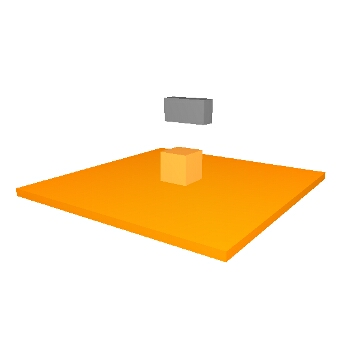
\includegraphics[width=3.5cm]{images/screenshots/box/1.jpg}
    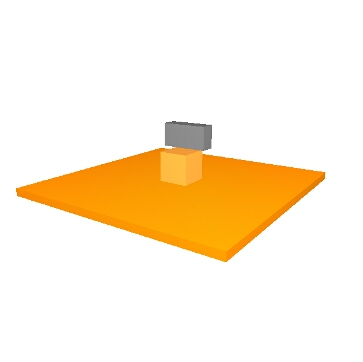
\includegraphics[width=3.5cm]{images/screenshots/box/2.jpg}
  }
  \qquad
  \subfloat[La boîte entre en contact avec le cube. Comme les points de
    contact sont excentrés par rapport à son centre de masse, une
    rotation s'en suit.]{
    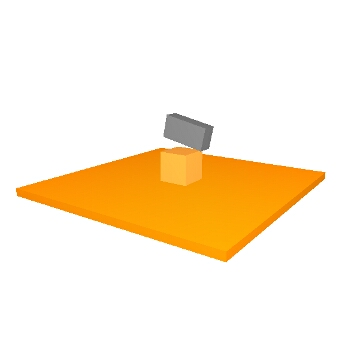
\includegraphics[width=3.5cm]{images/screenshots/box/3.jpg}
    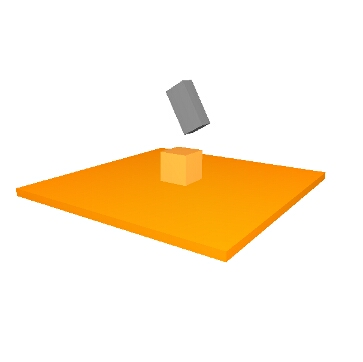
\includegraphics[width=3.5cm]{images/screenshots/box/4.jpg}
  }
  \qquad
  \subfloat[Au sommet de la trajectoire, la gravité reprend le dessus
    et la boîte redescend vers le cube.]{
    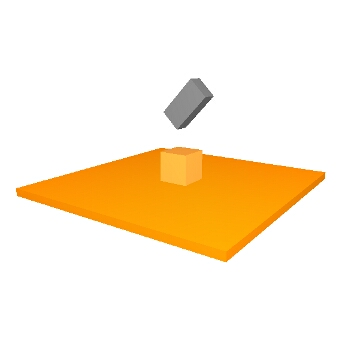
\includegraphics[width=3.5cm]{images/screenshots/box/5.jpg}
    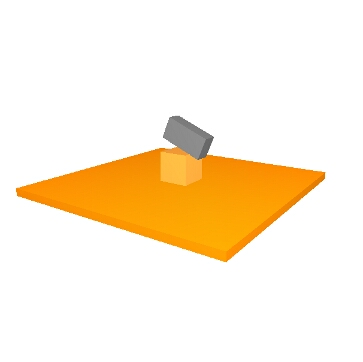
\includegraphics[width=3.5cm]{images/screenshots/box/6.jpg}
  }
  \qquad
  \subfloat[La boîte rebondit à nouveau sur le cube. Cette fois
    ci, sa vitesse angulaire la projette vers l'extérieur.]{
    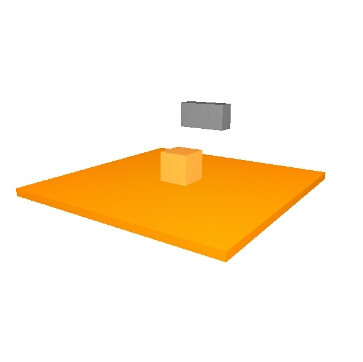
\includegraphics[width=3.5cm]{images/screenshots/box/7.jpg}
    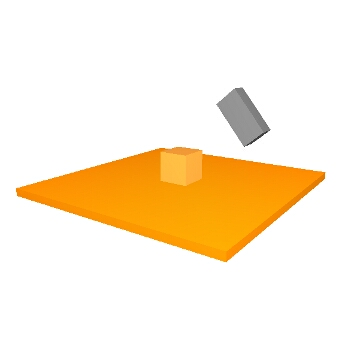
\includegraphics[width=3.5cm]{images/screenshots/box/8.jpg}
  }
  \qquad
  \subfloat[La boîte entre en collision avec le sol et rebondit
    pour finir sa course dans le vide.]{
    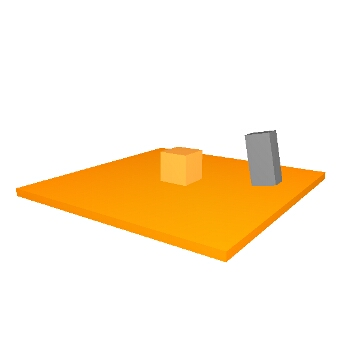
\includegraphics[width=3.5cm]{images/screenshots/box/9.jpg}
    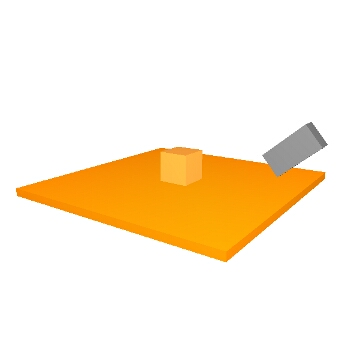
\includegraphics[width=3.5cm]{images/screenshots/box/10.jpg}
  }
  \qquad
  \caption{}
  \label{demoBox}
\end{figure}

\subsubsection*{Pachinko}

Le pachinko est un jeu de hasard japonais dans lequel des billes
métalliques sont lachées dans un parcours vertical parsemé de tiges
les déviant de leur trajectoire. Selon le chemin qu'elles empruntent,
de nouvelles billes peuvent être remportées, à la manière d'une
machine à sous.

Utilisons l'exemple de la machine à Pachinko pour illustrer les
capacités de notre moteur physique. Différentes étapes d'une chute de
billes sont commentées sur la figure \ref{demoPachinko}.


\begin{figure}
  \centering
  \subfloat[Les billes disposent initialement d'une vitesse nulle mais
    accélèrent rapidement vers le bas sous l'influence de la
    gravité. Elles passent la première rangée de tige sans qu'aucune
    collision ne s'opère.]{
    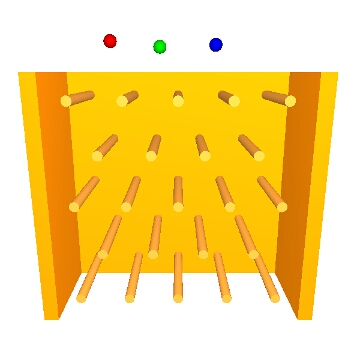
\includegraphics[width=3.5cm]{images/screenshots/pachinko/1.jpg}
    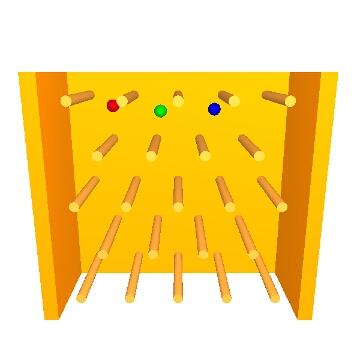
\includegraphics[width=3.5cm]{images/screenshots/pachinko/2.jpg}
  }
  \qquad
  \subfloat[La trajectoire de la bille rouge est déviée par une
    tige. Il en est de même pour la bille verte. Elles sont toutes
    deux projetées vers d'autres tiges. La bille bleue continue son
    chemin sans n'avoir encore touché aucune tige.]{
    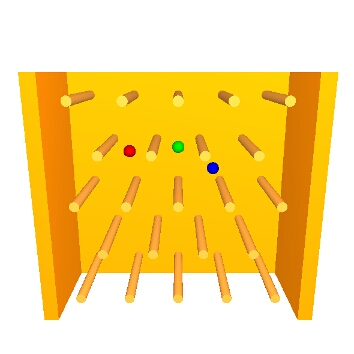
\includegraphics[width=3.5cm]{images/screenshots/pachinko/4.jpg}
    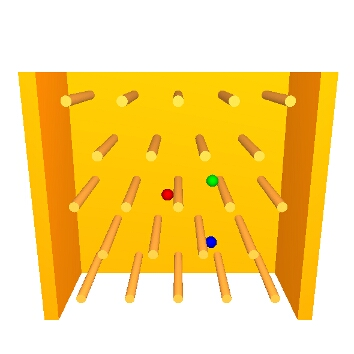
\includegraphics[width=3.5cm]{images/screenshots/pachinko/5.jpg}
  }
  \qquad
  \subfloat[La bille bleue est sortie de la machine à pachinko. Les
    deux autres billes se dirigent l'une vers l'autre jusqu'à ce
    qu'elles entrent en contact.]{
    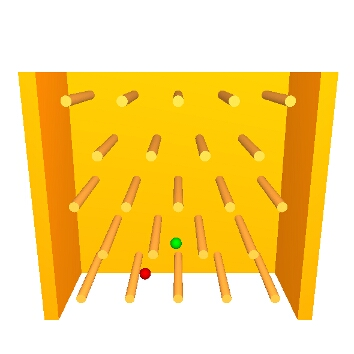
\includegraphics[width=3.5cm]{images/screenshots/pachinko/7.jpg}
    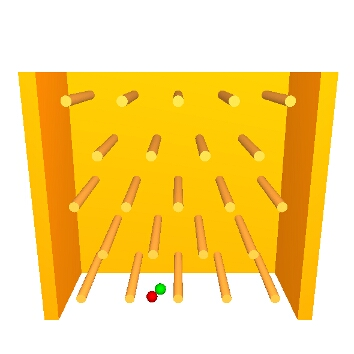
\includegraphics[width=3.5cm]{images/screenshots/pachinko/8.jpg}
  }
  \qquad
 \subfloat[Les billes restantes sont séparées et continuent leur
   course dans le vide.]{
    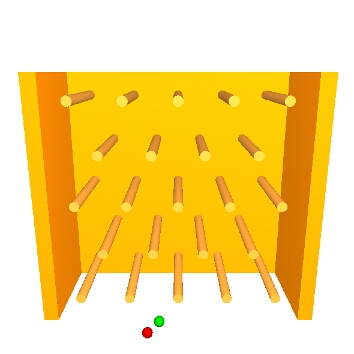
\includegraphics[width=3.5cm]{images/screenshots/pachinko/9.jpg}
  }
  \caption{}
  \label{demoPachinko}
\end{figure}

\subsection{Perspectives d'évolution}

\subsubsection{Tunneling}

Le moteur physique que nous concevons fonctionne par intégration
discrète et si aucun contrôle n'est effectué pour contrecarrer les
effets négatifs de cette caractéristique, on risque d'obtenir des
résultats imprécis ou pire, complètement éloignés de ce que l'on
retrouverait dans la réalité. On a par exemple vu plus tôt qu'une
phase de recherche dichotomique est nécessaire pour recaler les corps
à leur position réelle de contact lorsqu'une collision est détectée.

Néanmoins, une éventualité n'a pas été envisagée : que se passerait-il
si un objet en traversait entièrement un autre pendant un pas de temps
? On peut imaginer un objet $A$ lancé vers un autre objet $B$
fixe. \`A l'instant $t$, $A$ n'entre pas en collision avec $B$ mais se
dirige dans sa direction. \`A l'instant $t + \deriv t$, $A$ a
entièrement traversé $B$. \`A aucun de ces deux instants une collision
n'a été détectée et pourtant $A$ est impunément passé à travers
$B$. Le pas de temps utilisé pour réguler l'intégration du système
était donc trop faible pour s'assurer des collisions entre corps
évoluant à haute vitesse. Ce phénomène est appelé
\textit{tunneling}. \`A l'heure de l'écriture de ce rapport, le moteur
physique est sensible à ce genre de situation. Réellement, ce cas ne
se produit pas, puisque les simulations développées représentent des
situations terrestres qui font participer des forces d'opposition
telles que le frottement de l'air et donc les corps n'atteignent
jamais de vitesses démesurées. On souhaite tout de même disposer d'un
moteur physique solide et versatile, évaluons les possibilités qui
s'offrent à nous pour pallier ce problème.
\begin{figure}
  \centering
  \begin{tikzpicture}[scale=0.7, transform shape]
  \coordinate (AT1) at (0,0);
\coordinate (AT2) at (8,0);
\coordinate (B) at (6,0);

\draw node[fig,
  circle,
  minimum size=2cm,
  draw=bleu,
  dotted] (a1) at (AT1) {};

\node[fig,
  circle,
  minimum size=2cm,
  draw=bleu] (a2) at (AT2) {};
\node[fig,
  circle,
  minimum size=1cm,
  draw=rose] (b) at (B) {};



  \draw[->,thick,vert] (AT1) to node[black,auto] {$\deriv t$} (AT2);
\end{tikzpicture}

  \caption{Le phénomène du tunneling}
  \label{tunneling1}
\end{figure}

On pourrait envisager de diminuer la durée du pas de temps
d'intégration afin de diminuer le risque de tunneling, mais même si un
pas de temps faible améliore la qualité des résultats, il ne pourra
pas être indéfiniment réduit. Il est principalement limité par le
temps de calcul d'une mise à jour du système, puisqu'à partir du
moment o\`u $\deriv t$ est inférieur au temps moyen nécessaire à une
machine pour calculer une itération de la simulation, le programme
perdra son statut d'application temps réel.

Une technique usuellement admise est le lancer de rayons
(\textit{raycasting}) entre les points de la position de départ du
solide et les points de sa position d'arrivée. Si l'un des rayons
touche un autre corps, on sait qu'une collision aurait dû être
détectée et on peut revenir en arrière. Cette méthode présente
pourtant une faiblesse de taille, car le résultat de cette recherche
dépend directement de la concentration de rayons. Si on lance peu de
rayons, on risque de ne pas détecter les corps de petite taille et
donc de les traverser tandis qu'une concentration élevée de rayons
pourrait se réveler regrettable en terme de coûts de calcul.

\begin{figure}
  \centering
  \begin{tikzpicture}[scale=0.7, transform shape]
  \coordinate (AT1) at (0,0);
\coordinate (AT2) at (8,0);
\coordinate (B) at (6,0);

\draw node[fig,
  circle,
  minimum size=2cm,
  draw=bleu,
  dotted] (a1) at (AT1) {};

\node[fig,
  circle,
  minimum size=2cm,
  draw=bleu] (a2) at (AT2) {};
\node[fig,
  circle,
  minimum size=1cm,
  draw=rose] (b) at (B) {};



  \path[rayon] (a1.north) -- (a2.north);
  \path[rayon] (a1.west) -- (a2.west);
  \path[rayon] (a1.north west) -- (a2.north west);
  \path[rayon] (a1.south) -- (a2.south);
  \path[rayon] (a1.south west) -- (a2.south west);
\end{tikzpicture}

  \caption{Lancer de rayons pour la détection de tunneling}
  \label{tunneling2}
\end{figure}

La technique de la détection de collision continue (\textit{continuous
  collision detection}) permet de contrôler de façon certaine tout
phénomène de tunneling. L'idée est la suivante : soit deux corps $A$
et $B$ dont l'on veut détecter l'éventuelle collision. On construit
deux volumes fantômes $C_A$ et $C_B$ englobant tous les points par
lesquels passent respectivement $A$ et $B$ entre deux
intégrations. Ces volumes n'interviendront pas dans les collisions des
autres objets de la simulation, et on vérifie simplement s'ils entrent
tous deux en collision. Si tel est le cas, alors on sait qu'il est
possible qu'un tunneling se soit produit et on peut revenir en arrière
jusqu'à ce que le problème soit résolu. Pour accélérer cette phase, il
est envisageable d'utiliser des boîtes englobantes de la même façon
que lors de la détection grossière de collision. L'un des avantages
majeurs de cette méthode, en plus de sa certitude de ne manquer aucun
tunneling, est sa simplicité de mise en place puisque toutes les
routines de détection et de retour en arrière utilisées ont déjà été
écrites et entrent en jeu dans le fonctionnement de base du moteur
physique.

\begin{figure}
  \centering
  \begin{tikzpicture}[scale=0.7, transform shape]
  \coordinate (AT1) at (0,0);
\coordinate (AT2) at (8,0);
\coordinate (B) at (6,0);

\draw node[fig,
  circle,
  minimum size=2cm,
  draw=bleu,
  dotted] (a1) at (AT1) {};

\node[fig,
  circle,
  minimum size=2cm,
  draw=bleu] (a2) at (AT2) {};
\node[fig,
  circle,
  minimum size=1cm,
  draw=rose] (b) at (B) {};



  \coordinate (a1n) at ($(a1.north)+(0,0.2)$);
  \coordinate (a2s) at ($(a2.south)+(0,-0.2)$);

  \draw[gris] (a1n) arc (90:270:1.2cm) --
  (a2s) arc (-90:90:1.2cm) --
  (a1n);
\end{tikzpicture}

  \caption{Boîtes englobantes pour la détection de tunneling}
  \label{tunneling3}
\end{figure}

\subsubsection{Partitionnement de l'espace}

Comme mis en avant tout au long de ce rapport, on cherche à concevoir
un moteur physique dont la rapidité d'éxécution est un facteur
déterminant. Dans cette optique, il est primordial d'optimiser les
routines géométriques entrant en jeu mais aussi d'éviter leur
exécution inutile dès que possible. La détection des collisions entre
les corps qui peuplent notre système se déroule en deux étapes : une
détection grossière visant à vérifier de façon économique si deux
objets se touchent et une détection fine servant à confirmer ou à
infirmer de façon sûre ce résultat. Bien que la détection grossière
soit peu coûteuse en termes de calcul, elle est éxécutée pour $n$
corps au minimum $\frac{n(n-1)}{2}$ fois à chaque itération, et ce
sans compter les détections de collision exécutées pendant la
recherche dichotomisuqe de l'état de contact. Pourtant, il est très
souvent inutile de détecter si deux objets sont en situation
d'interpénétration, par exemple lorsque la distance les séparant est
grande. Il serait tout à notre avantage d'ajouter au moteur une couche
supplémentaire tenant compte de ces disparités spatiales pour
accélérer la phase de détection de collision.

Le principe général du partitionnement de l'espace (\textit{spatial
  partitioning}) est de subdiviser l'environnement de la simulation en
sous-espaces. La répartition des corps dans ces sous-espaces dépend
bien évidemment de leur position dans le repère global mais aussi du
volume qu'ils occupent. On est certain que seules les entités
appartenant à un même sous-espace peuvent interagir entres elles, on
dispose donc d'une aide quant au choix des objets entre lesquels
vérifier si collision il y a.

Sous sa forme la plus simple, le partitionnement de l'espace prend la
forme d'une grille de taille fixe dans les cases de laquelle les corps
de la simulation sont répartis. L'aspect statique d'une telle
structure présente plusieurs inconvénients majeurs, notamment le fait
que le gain de performance variera fortement selon le nombre d'objets
considérés, leur taille et la finesse de la grille. Par exemple, si
une grille a des cases trop grandes, chacune contiendra de nombreux
objets et le gain de performance sera peu flagrant. Si au contraire
les cases de la grille sont trop petites, les plus grands objets ne
pourront pas rentrer dans leur intégralité à l'intérieur d'une unique
case. Une solution à ce problème est de ranger un même objet dans
plusieurs cases adjacentes de la grille, mais une fois encore, si des
corps sont démultipliés de la sorte, le temps de maintenance d'une
telle structure sera augmenté.

Une variante plus subtile de partitionnement de l'espace est
l'utilisation d'\textit{octrees} (\textit{quadtrees} en deux
dimensions) \cite{millington}. Cette structure de données prend la forme d'un arbre
représentant l'espace à subdiviser. Chaque n\oe ud de l'arbre possède
huit fils, chacun correspondant à un octant du volume de leur père. La
racine de l'arbre est associée au volume complet de l'environnement
que l'on souhaite diviser. Lorsqu'un corps est introduit dans la
simulation, il faut le ranger dans l'arbre. Pour ce faire, on part de
la racine et on descend récursivement jusqu'à une feuille de l'arbre
en se guidant dans les embranchements selon la position et le volume
de l'objet à insérer. L'octree n'est pas nécessairement équilibré et
plus une zone contient de corps et plus elle pourra être subdivisée.

Cette structure sert à stocker les corps de la simulation, et si nous
l'implémentions elle remplacerait la liste qui contient nos objets et
dont l'ordre est actuellement arbitraire. Elle devient
particulièrement intéressante lors de la phase de détection de
collision car il n'est plus désormais nécessaire de tester tous les
corps deux à deux; il suffit de vérifier les collisions entre les
corps du même sous-espace, autrement dit avec tous ceux contenus dans
la même feuille.

\section{Conclusion}

Le but de ce projet était d'étudier et d'implémenter un moteur
physique de base simulant le comportement mécanique de corps
rigides. Pour ce faire, nous nous sommes basés sur une modélisation
des lois de Newton utilisant forces et impulsions. De nombreux choix
concernant les solutions utilisées sont justifiés par la contrainte du
temps réel. Désirant néanmoins une modélisation aussi précise que
possible, il a été nécessaire d'implémenter des méthodes de correction
permettant de conserver à la fois cohérence spatiale et cohérence
temporelle.

Le problème récurrent de ce type d'application est la stabilité, non
pas au sens de la stabilité logicielle, mais plutôt en celui de la
stabilité des configurations atteintes. Afin d'obtenir des simulations
équilibrées, des seuils de tolérance calibrés ont dû être employés à
différentes étapes du travail du moteur physique, comme lors de la
phase de détection de collision et de correction. \`A l'heure
actuelle, il est tout de même difficile d'obtenir certaines
configurations, notamment des empilement de solides, cas dans lequel
les collisions de tous les objets au repos apparaissent au même
instant. Une solution serait de mettre en place une technique de
correction indépendante du temps. Elle déterminerait la profondeur de
pénétration associée à une collision et recalerait les objets en
modifiant uniquement leur position. On perdrait la cohérence
temporelle et on ignorerait les variations d'orientation entre l'état
au moment de la détection et l'état après correction, mais cette
approximation augmenterait les capacités du moteur physique tout en
conservant l'atout du temps réel.

D'autres modélisations existent et sont fondées sur la résolution de
systèmes linéaires pour gérer les contacts. \`A chaque mise à jour, on
converge progressivement vers une configuration satisfaisante. Il
n'est dans ce cas pas gênant que des interpénétrations existent tant
qu'elles restent imperceptibles. La stabilité fournie par ce genre de
méthode justifie à elle seule l'emploi de telles techniques. Il serait
intéressant de les étudier à l'avenir.

\section*{Notes}

Je tiens à remercier tout particulièrement Jean-Luc Ponty, mon tuteur
dans le cadre de ce projet, pour l'attention qu'il lui a apportée
ainsi que pour son aimable correction.

Je remercie aussi Eric Sanlaville, responsable de la première année de
master Informatique, qui a autorisé la poursuite de ce projet bien
qu'il soit issu d'un v\oe u personnel.

Un grand merci à Maureen et à Florent pour les corrections et conseils
qu'ils m'ont prodigués. \\

Le code source du moteur physique est hébergé sur Github.com et est
accessible à l'adresse \url{http://github.com/merwaaan/tperigidbody/}.


\printbibliography

\end{document}
